\subsection{Detector $Q$ resolution} \label{subsec:qres}
To properly azimuthaly integrate the images taken from the detector the $Q$ resolution of the pixels must be calculated.
Integrating using even bins will cause pixels which are not on the same ring to be binned together, causing the incorrect value of $I(Q)$ to be obtained and a larger standard deviation in the integrated data.
To properly calculate the $Q$ resolution the resolution of each of the pixels in $2\theta$ must be calculated.
\begin{figure}
    \centering
    \begin{tikzpicture}
        \draw (0,0) node[anchor=north]{$A$}
          -- (4,0) node[anchor=north]{$C$}
          -- (4,4) node[anchor=east]{$B$}
          -- cycle;
        \draw (0,0) node[anchor=north]{$A$}
          -- (4,0) node[anchor=north]{$C$}
          -- (4,6) node[anchor=south]{$B'$}
          -- cycle;
    \end{tikzpicture}
    \caption{Scattering onto a flat detector}
    \label{fig:scattering_digram}
\end{figure}
Figure \ref{fig:scattering_digram} shows the scattering of x-rays onto a flat image plate detector.
In this diagram the bottom of the $n$th pixel is $B$ while the top is $B'$.
The resolution of this pixel in $2\theta$ is $\angle BAC - \angle B'AC$.
Thus the resolution, calculated from the distances is
\begin{equation}
\Delta 2 \theta = \arctan{\frac{b}{d}} - \arctan{\frac{t}{d}}
\end{equation}
where d is the sample to detector distance, b is the distance to the bottom of a pixel, and t is the distance to the top of that pixel.
Note that these distances need to have been corrected for detector tilt and rotation.
Thus the resolution of a pixel in $Q$ is
\begin{equation}
\Delta Q = \frac{4\pi(\sin{\arctan{\frac{b}{d}}} - \sin{\arctan{\frac{t}{d}}})}{\lambda}
\end{equation}
where $\lambda$ is the x-ray wavelength.

For a Perkin Elmer image plate, like the one used at the NSLS-II's XPD and the APS's 11-ID-B, the resolution function is shown in \ref{fig:res_func}.
For the same detector the number of pixels per $Q$ is shown in \ref{fig:pixel_hist}
\begin{figure}[!ht]
  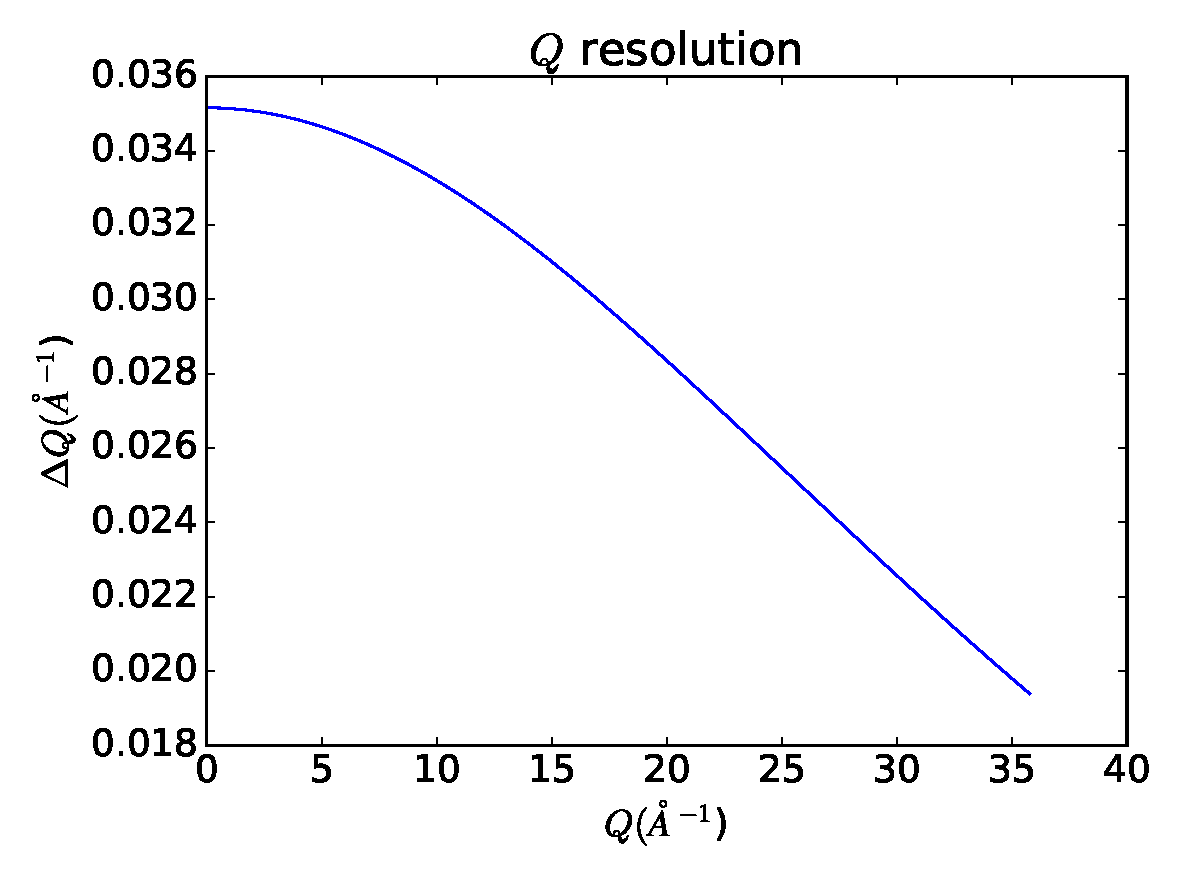
\includegraphics[width=\textwidth]{res}
\caption{$Q$ resolution as a function of $Q$.}
\label{fig:res_func}
\end{figure}

\begin{figure}[!ht]
  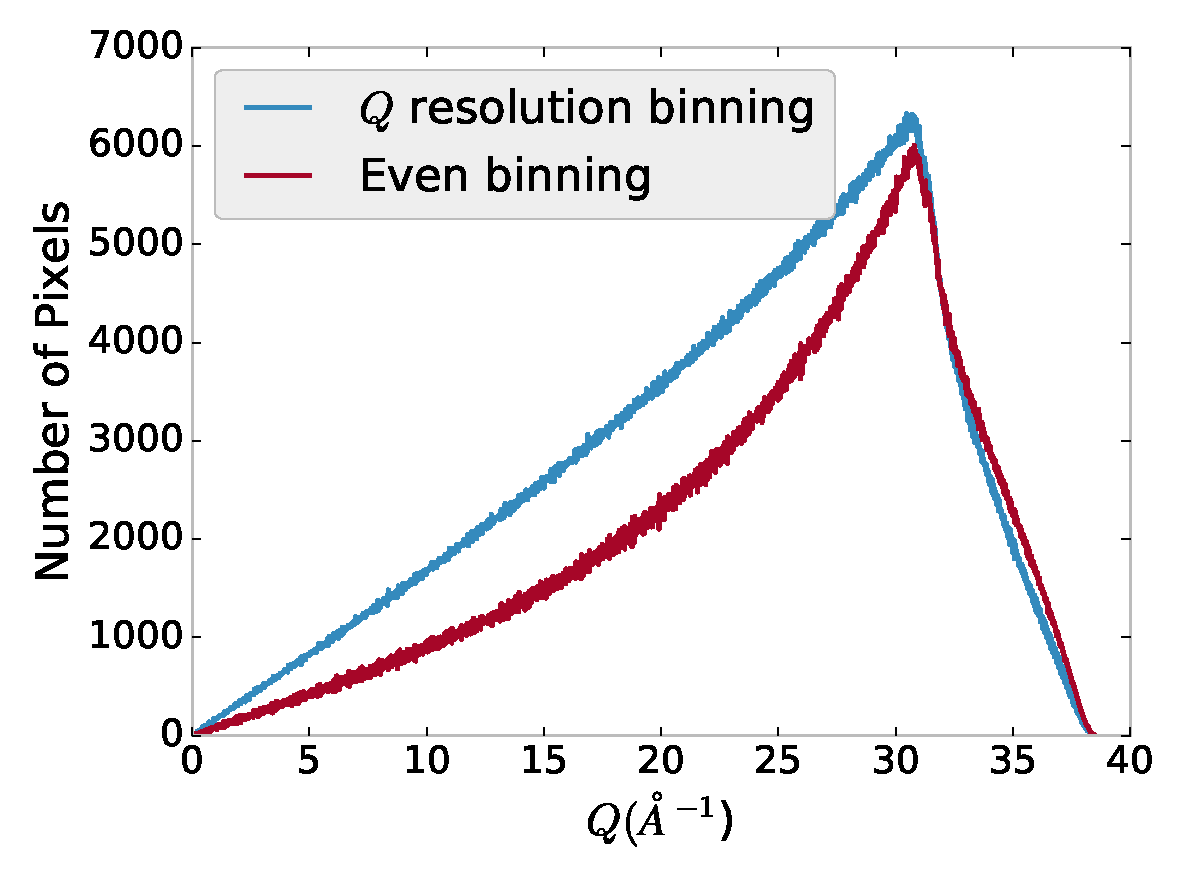
\includegraphics[width=\textwidth]{pixels}
\caption{Number of pixels as a function of $Q$, binned at the $Q$ resolution of the detector.}
\label{fig:pixel_hist}
\end{figure}